\chapter{Deployment}
\section{Introduction}
\section{Code used in the pipeline}
For testing the group decided on using OWASPs Juice Shop, which is a deliberately vulnerable web application that is designed to help developers and others to learn about web applications security concepts. The code is designed to simulate a real-world application by having common vulnerabilities within the code. The intention is to encourage users to find these vulnerabilities and to exploit them and increase the understanding of web application security \cite{owaspJuiceShop}.
The code in the OWASP Juice Shop is open source code on GitHub and is written in TypeScript, which uses a Node.js server and Angular for \gls{front-end}. \cite{owaspJuiceShopCode}
The code contains of different vulnerabilities, including SQL injections, cross-site scripting and many others. 
Overall, OWASP Juice Shop encourages users to improve their skills and it allows for customization and adaption for specific needs from the users. 

\begin{comment}
\section{Security when coding}
Here we can write something about security while coding, maybe get CodeQL to work so we can test that idk??? Maybe out of scope
\end{comment}

\section{Security when pushing to GitHub}

%\subsection{Access control}
%Something about access control

\subsection{Branch protection}
Branch protection rules are easy to enable in GitHub. It is done for each individual repository. GitHub has different rules one can enable, which are explained in \ref{branchprotection}.
\begin{comment}
Can easily be enabled in GitHub. Branch protection rules are enables for individual repositories, different repos have different structures and branches. Under settings->Code and automation->Branches you can add branch protection rules. You just enable the ones you want. 
\end{comment}

\subsection{Signed commits}
For signing commits in GitHub, one can either use an SSH or GPG key. These need to be generated and connected to the users GitHub account. By adding this security measurement, it increases the authentication of the developer. 
\\~\\
How to generate and connect a key to a GitHub account is done by following the steps GitHub has provided:\\
https://docs.github.com/en/authentication/managing-commit-signature-verification/signing-commits
\begin{comment}
Generate a new ssh key:
\begin{tcolorbox}
\begin{verbatim}
$ ssh-keygen -t ed25519 -C "your_email@example.com"
\end{verbatim}
\end{tcolorbox}

You will have to name the file where the public and private key will be saved, let´s call it "example\_key" and assume it was added with the path "\$sim/.ssh"
\\~\\
Add this key to the ssh-agent:\\
\begin{tcolorbox}
\begin{verbatim}
$ ssh-add ~/.ssh/example\_key
\end{verbatim}
\end{tcolorbox}

After this, the key must be added to the GitHub account. Settings->Access->SSH and GPG keys. You add a new SSH key, give it a name, make it a signing key and add the public key.



\begin{figure}[H]
    \centering
    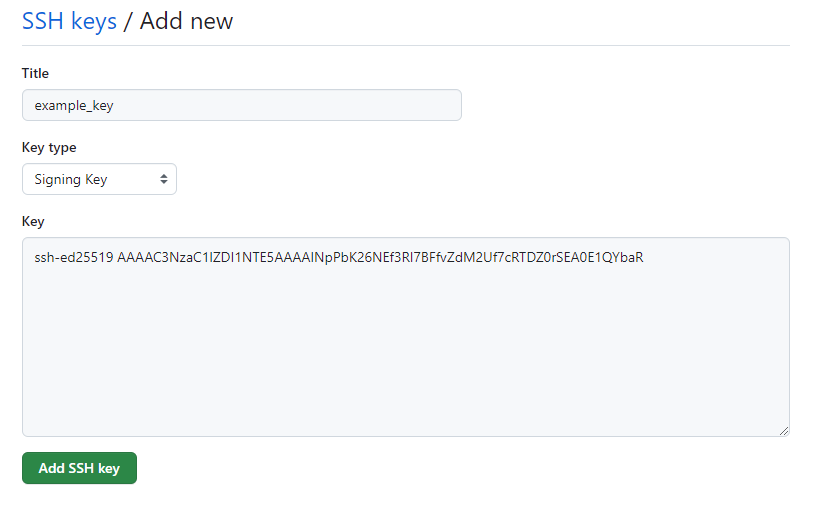
\includegraphics{Images/ssh-key.png}
    \caption{Adding a new SSH key in GitHub}
    \label{fig:ssh_key_github}
\end{figure}

In order to protect your signature from someone who has gotten access to your SSH key, it can be added a passphrase:
\\~\\
\begin{tcolorbox}
\begin{verbatim}
$ ssh-keygen -p -f ~/.ssh/example\_key
\end{verbatim}  
\end{tcolorbox}

Now the key needs to be used for signing. First configure Git to use ssh as key signature:
\begin{tcolorbox}
\begin{verbatim}
$ git config --global gpg.format ssh
\end{verbatim}  
\end{tcolorbox}

Then git needs to know which key you want for signing\\
\begin{tcolorbox}
\begin{verbatim}
$ git config --global user.signingkey ~/.ssh/example_key.pub 
\end{verbatim}
\end{tcolorbox}

Only thing left is signing you commits. This is done by adding the parameter "-S" in your commit:

\begin{tcolorbox}
\begin{verbatim}
$ git commit -S -m "This is a commit
\end{verbatim}
\end{tcolorbox}
When this is done, you have to enter your passphrase, and the commit will be verified.

\begin{figure}[H]
    \centering
    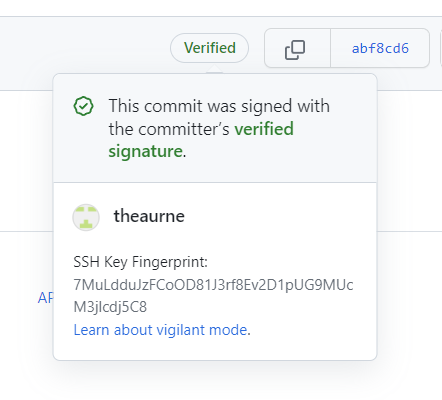
\includegraphics{Images/verified-commit.png}
    \caption{Verified commit in GitHub}
    \label{fig:verified-commit}
\end{figure}
\end{comment}

\section{Security when in Git}
%Code scans, dependabot and secret scanner needs to be enabled. Dependabot only needs to be enabled, and does not require any configuration. 

\subsection{Configuring CodeQL}
When configuring CodeQL in a GitHub repository, one can either use a default setup or configure it themselves.CodeQL i suggested as a default in the code scanning tool configurations.
In the chosen repository, configure a code scanning tool. Here, CodeQL is suggested as a default. Configuring the default is easy, just add the YAML file, it will detect the used language. Can also configure the yaml file. 

\subsection{Dependabot}
%Enable dependabot in the security settings. Very intuitive and easy to do, user friendly :D

\subsection{Secret Scanning}


\section{AWS}
\subsection{Terraform}
Terraform\footnote{https://www.terraform.io/} is a tool for automating resource configurations. In this case, Terraform is used to configure the AWS CodePipeline. \\
%Write about automation, idempotent etc.. \\
%In the code: specifies git repo, write build commands, apply it \\
\newpage
%\begin{lstlisting}[style=terraform, caption= Terraform %example, captionpos=b]
\begin{comment}
\begin{verbatim}
terraform {
  required_providers {
    aws = {
      source  = "hashicorp/aws"
      version = "~> 4.16"
    }
/**
    snyk = {
      source = "snyk/snyk"
      version = ">= 1.0.0"
    }
    */
  }

  required_version = ">= 1.3.0"
}

provider "aws" {
  profile = "default"
  region  = "eu-north-1"
}

\end{verbatim}
%\end{lstlisting}
\end{comment}
%Include code snippets?

\subsection{Signed Artifacts}


\subsection{OWASP Zap}


\subsection{Penetration testing}

\section{Security after deployment}
\begin{comment}
   -WAF og NAC tools \\
- monitoring, logging and alerting \\
- AWS cloudwatch \\
- Utføre regelmessige pentester/aws inspector  \\
- AWS WAF, AWS shield, 
- AWS security hub 
\end{comment}

